\documentclass[12pt]{article} % Default font size is 12pt, it can be changed here

\usepackage[utf8]{inputenc} % utf8 encoding
\usepackage{geometry} % Required to change the page size to A4
\geometry{a4paper} % Set the page size to be A4 as opposed to the default US Letter

\usepackage{graphicx} % Required for including pictures
%\usepackage{asmath} % Required for math functions with cases 
\usepackage{float} % Allows putting an [H] in \begin{figure} to specify the exact location of the figure

\linespread{1.2} % Line spacing

%\setlength\parindent{0pt} % Uncomment to remove all indentation from paragraphs

\graphicspath{{pictures/}} % Specifies the directory where pictures are stored

\usepackage{listings} % To be able to have code in text
\usepackage{color} % To be able to have colors

\definecolor{codegreen}{rgb}{0,0.6,0}
\definecolor{codegray}{rgb}{0.5,0.5,0.5}
\definecolor{codepurple}{rgb}{0.58,0,0.82}
\definecolor{backcolour}{rgb}{0.95,0.95,0.92}
 
\lstdefinestyle{codestyle}{
    backgroundcolor=\color{backcolour},   
    commentstyle=\color{codegreen},
    keywordstyle=\color{magenta},
    numberstyle=\tiny\color{codegray},
    stringstyle=\color{codepurple},
    basicstyle=\footnotesize,
    breakatwhitespace=false,         
    breaklines=true,                 
    captionpos=b,                    
    keepspaces=true,                 
    numbers=left,                    
    numbersep=5pt,                  
    showspaces=false,                
    showstringspaces=false,
    showtabs=false,                  
    tabsize=2
}
 
\lstset{style=codestyle}

\begin{document}

%----------------------------------------------------------------------------------------
%   TITLE PAGE
%----------------------------------------------------------------------------------------

\begin{titlepage}

\newcommand{\HRule}{\rule{\linewidth}{0.5mm}} % Defines a new command for the horizontal lines, change thickness here

\center % Center everything on the page

\textsc{\LARGE Lund University, Faculty of Engineering}\\[1.5cm] % Name of your university/college
\textsc{\Large EDAF05}\\[0.5cm] % Major heading such as course name
\textsc{\large Algorithms, data structures, and complexity}\\[0.5cm] % Minor heading such as course title

\HRule \\[1cm]
{ \huge \bfseries Summary of EDAF05}\\[0.4cm] % Title of your document
\HRule \\[1.5cm]

\emph{Author:} Fred \textsc{Nordell} % Your name

{\large \today}\\[3cm] % Date, change the \today to a set date if you want to be precise

%\includegraphics{Logo}\\[1cm] % Include a department/university logo - this will require the graphicx package

\vfill % Fill the rest of the page with whitespace

\end{titlepage}

%----------------------------------------------------------------------------------------
%   TABLE OF CONTENTS
%----------------------------------------------------------------------------------------

\tableofcontents % Include a table of contents
\lstlistoflistings % Include a table of lstlistings
\listoffigures % Include listing of figures
\listoftables

\newpage % Begins the essay on a new page instead of on the same page as the table of contents 


\section{Algorithms} % Major section

This section will describe the different problems and algorithms covered in the course.

\begin{table}[h!]
\centering
\begin{tabular}{| c | c | c |}
    \hline
    Lab & Area & Comment \\
    \hline \hline
    Stable marriage & Matching & Gale-Shapely \\
    Word ladders & Graph connection & Find connection between words $s$ and $t$ \\
    Spanning USA & Greedy & Find the MST, Prim's or Kruskal's \\
    Closest pair & Divide and conquer & Find the closest pair \\
    Gorilla & Dynamic programming & String alignment \\
    Railroad & Network flow & Find minimal cuts \\
    \hline
\end{tabular}
\caption{Table of labs and their corresponding algorithm}
\label{table: 1}
\end{table}

\subsection{Stable Marriage} % Sub-section
Given two sets $X = {x_{1}, x_{2}, \dots x_{n}}$ and $Y = {y_{1}, y_{2}, \dots y_{n}}$ a matching $M$ is a set of pairs $(x_{i}, y_{j})$ such that an $x \in X$ and an $y \in Y$ appear in most one pair. Thus it follows that a matching does not let anybody have multiple partners.

\par If the size of $M$ is $n$ it is called a \textbf{perfect matching} (All members of $X$ and $Y$ were matched). Hoverer a perfect match is insufficient. All $x$ and $y$ have a preferred list, sorted in descending order, of the opposite set. The matching $M$ is considered \textbf{unstable} if it contains to pairs where they would rather switch partners. \textit{i.e.}\\
$x_{i}$ prefers $y_{j}$ and $y_{j}$ prefers $x_{i}$ \\
or \\
$y_{p}$ prefers $x_{q}$ and $x_{q}$ prefers $x_{p}$ \\
Is it always possible to find a stable matching with no unstable pairs?

\subsubsection{The Gale-Shapely algorithm}
As each person has a preferred list of partners each $x$ just needs to remember the position in the list. But as $y$ has to accept $y$ has to check if $x$ is before the current matched $x_{y}$. This may need $O(n)$ operations. A naive implementation of this algorithm may have a time complexity of $O(n^3)$ as each $x$ tries to match with each $y$ and each ask take $O(n)$ time. To reduce time complexity each $y$ should not save a preference list, instead they should save an inverted list. Thus \texttt{[3, 2, 4, 1]} means that $x_{1}$ comes at position 3 and $x_{4}$ comes at position 1. This reduces the operation to constant time. Below is a Java implementation of the Gale-Shapely algorithm.

\begin{lstlisting}[language=Java]
public String match() {
        for(Person p: persons) {
            if(p.getId() % 2 == 0) {
                y.add(p);
            } else {
                x.addLast(p);
            }
        }
        while(x.size() > 0) {
            Person m = x.removeFirst();
            int w = (m.getPrefered()/2)-1;
            if(y.get(w).matched == null) {
                y.get(w).matched = m;
                m.matched = y.get(w);
            } else if(y.get(w).compareMatched(m)) {
                x.addLast(y.get(w).matched);
                y.get(w).matched = m;
                m.matched = y.get(w);
            } else {
                x.addLast(m);
            }
        }
        StringBuilder sb = new StringBuilder();
        for (Person w : y) {
            sb.append(w.matched.name + " -- " + w.name + "\n");
        }
        return sb.toString();
    }
\end{lstlisting}

\subsection{Graphs} % Sub-section
\begin{figure}[H]
\center{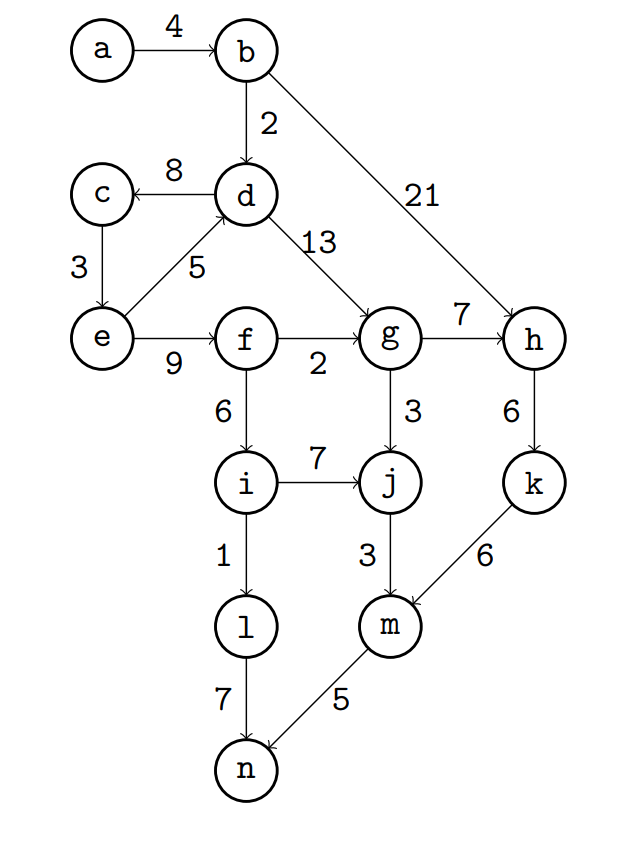
\includegraphics[width=0.5\linewidth]{graph}}
\caption{Example graph.}
\label{exGraph}
\end{figure}
A graph is a set of nodes $V$ and a set of edges $E$. Edges connects nodes together. A graph which edges you are able to follow from one to another but not backwards is called a \textbf{directed graph}. In contrary a graph whose edges connections both to and from a node is called an \textbf{undirected graph}. An undirected graph is \textbf{connected} if there is a path between every pair of nodes. A \textbf{cycle} is a path which terminates in the start node. In a connected graph there is no unreachable nodes. A graph is said to be disconnected if there exists two nodes in $G$ such that no path in $G$ has those two nodes as endpoints. A graph with one vertex is connected. An edgeless graph with two or more vertices is disconnected.

\subsubsection{Bipartite graphs}
A bipartite graph is a graph that can be coloured with two colours such that every edge connects two nodes with different colours.

\begin{figure}[H]
\center{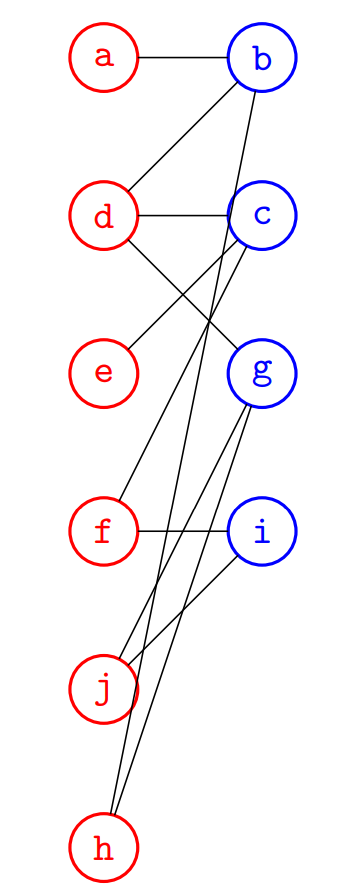
\includegraphics[width=0.5\textwidth,height=0.5\textheight,keepaspectratio]{bipartite}}
\caption{Example bipartite graph.}
\label{exBiGraph}
\end{figure}

\subsubsection{BFS and DFS}
The problem is to find a path from $s$ to $t$. There are two different approaches, breath first and depth first. Depth first explores all possible branches first and the n backtracks to find the shortest path if there is any. Breath first is the opposite, you explore the closest nodes first and then explore one level deeper. Basically like ripples on a lake, start close and propagate outwards until you hit your target.

\par Time complexity of DFS is $O(V + E)$ and of BFS is $O(V + E)$, how neat.

\begin{lstlisting}[language=Python, caption=Recursive DFS in Python]
def DFS(G,v):
    label v as discovered
    for all edges from v to w in G.adjacentEdges(v) do
        if vertex w is not labelled as discovered then
            recursively call DFS(G,w)
\end{lstlisting}

\begin{lstlisting}[language=Python, caption=BFS in Python/pseudo]
def BFS(G,v,target):
    create empty set Visited
    Q = new Stack()
        Q.append(v)                      
        while Q is not empty:
            current = Q.pop()
            if current.value == target:
                    return current
            for each node n that is adjacent to current:
                    if n is not in Visited:
                    Q.enqueue(n)
\end{lstlisting}

\subsection{Greedy algorithms} % Sub-section
The definition is not trivial. Main idea is to make the best local decision at a potential cost at the global level. Herein lies the problem of finding the rule which solves the problem optimally. There are two ways we can prove optimality. 
\begin{enumerate}
\item If the greedy algorithm is at least as good as an optimal solution we know it is also optimal
\item Exchange argument -- transform the output of an optimal algorithm to the output of the greedy algorithm
\end{enumerate}

\subsubsection{Greedy graph algorithms}
How do we find the shortest path in a given graph? to every other node? Can we find this efficiently? Edges have weights which can be both negative and positive (although easier with positive).

\subsubsection{Dijkstra's algorithm}
Given a directed graph $G(V, E)$ a weight function $w: E -> R$ and a node $s \in V$ Dijkstra's algorithm computes the path to every other node. To find the path to a specific node traverse backwards until v. Alternately implement a condition where the algorithm ends when the target is found.
\par Assume $n$ nodes and $m$ edges, the running time is $O(m \cdot log(n))$. Below is a python/pseudo-code implementation.

\begin{lstlisting}[language=Python, caption=Dijkstra's in pseudo/Python]
node n = (value, edges)
def Dijkstra(G,n,target):
    n.value = 0; #sets the start nodes value to 0, All other nodes should have inf as value. 
    Visited = {}
    while n != target:
        for Edges connected to n not in Visited:
            if n.value + edge.value < edge.end.value:
                edge.end.value= n.value + edge.value
        Visited.append(n)
        n = nextNode #pick out a node not in visited connected to n
    return n.value
\end{lstlisting}

\subsubsection{Prim's algorithm}
Assume the nodes are cities and a country wants to connect the cities to a electrical network. We want to find a subset of edges where all cities are connected at minimal cost i.e. we want to find the \textbf{minimum-weight spanning tree}.
\par Given a undirected graph $G(V,E)$ $T \subseteq E$ and $(V, T)$ is a tree it is called a \textbf{spanning tree} of $G(V, E)$. If the edge costs are minimized, it is a \textbf{MST}. Prim's algorithm is similar to Dijkstra's as it builds one $MST$. At the core there is the problem if it is safe to add an edge. A partition $(S, V - S)$ of the nodes $V$ is called a \textbf{cut}. An edge $(u, v)$ crosses the cut if $u \in S$ and $v \in V - S$, that $u$ and $v$ are in different parts of the partition. How to determine safeness is in lecture slides. The running time of Prim's is $O(m \cdot log(n))$

\begin{lstlisting}[language=Scala, caption=Prim's in Scala]
class Node(id: String, var cost: Int = Int.MaxValue, var leastEdge: Edge = null) extends Ordered[Node]{
  var edges = scala.collection.mutable.PriorityQueue[Edge]()

  def compare(that: Node) = cost compare that.cost

  def addEdge(from: Node, to: Node, weight: Int): Unit = {
      edges.enqueue(new Edge(from, to, weight))
  }
  override def toString: String = id
}
class Edge(val from: Node, val to: Node, val weight: Int) extends Ordered[Edge]{

    def compare(that: Edge) = that.weight compare weight

    override def toString: String = from + "<-->" + to + " ("+ weight +")"

}
def prim(g: List[Node]): scala.collection.mutable.HashSet[Node] = {
    var mst_nodes = scala.collection.mutable.HashSet[Node]()
    val pq = new java.util.PriorityQueue[Node](g.asJava)
    pq.peek().cost = 0
    while(!pq.isEmpty) { //O(n)
      val node = pq.poll()
      mst_nodes += node
      node.edges.foreach(e => //snitt O(m/n)
        if (!(mst_nodes contains e.to)) {
          if (e.to.cost > e.weight) {
            e.to.cost = e.weight
            e.to.leastEdge = e
            pq.remove(e.to) //log(n)
            pq.offer(e.to)
          }
        }
      )
    }
    return mst_nodes //multiply them => O(m*log(n))
  }
\end{lstlisting}

\subsubsection{Kruskal's algorithm}
Kruskal's algorithm builds a forest that later becomes one MST. The running time is $O(e \cdot log(v))$ where $v$ is the vertices and $e$ is the edges in the graph $G(V, E)$. 

\begin{lstlisting}[language=Python, caption=Kruskal in python]
def kruskal(V,E):
sort(E) //Sorts E, low to high
forest = {}
while E.length != 0:
    edge = E.pop()
    if edge has no endpoint in the forest:
        forest.append(edge)
return forest
\end{lstlisting}

\subsection{Divide and Conquer}
Divide and conquer is the technique of dividing a hard problem to multiple easier problems and then solving those. Suppose we have a problem which can be solved in $O(n^2)$ time, if we divide this problem into two sub-problems in linear time and save those problems and then combine the results in linear time the running time becomes $O(n \cdot log(n))$. Some examples include Merge sort, calculation of Fibonacci numbers or finding the largest perfect sub-tree in a binary search tree.

\begin{lstlisting}[language=Python, caption=Fibbonaci in Python]
#find the n:th number in the Fibonacci sequence.
def fibonacci(number n):
    if n =< 1:
        return fibonacci(n-1) + fibonacci(n-2)
    else:
        return 1
\end{lstlisting}
\begin{lstlisting}[language=Python, caption=Perfect sub-tree in BST in Python]
def func(node n):
    if(n!=None):
        tuple = (func(n.left),func(n.right))
        MyMax = 1+ min(tuple[0],tuple[1])
        TotalMax = max(MyMax,tulp[0],tuple[1])
        return (myMax,TotalMax);
    else:
        return (0,0)
\end{lstlisting}

\subsection{Dynamic programming} % Sub-section
Dynamic programming is closely related to divide and conquer but with some crucial differences. In divide and conquer we solve \textbf{independent} sub-problems but in Dynamic programming we solve \textbf{overlapping} sub-problems. The idea is to avoid computing already computed sub-problems, but rather to store the already computed sub-problems and access that when the same problems comes up again. This technique of storing the solutions is called \textbf{Memoization}. Furthermore we can categorize this problem solving method into two categories, the \textbf{top-down} and \textbf{bottom-up} approaches. Top-down is when one would start with a large problem and recursively using the smaller sub-problems to solve the problem at hand. Bottom-up on the other hand would solve the sub-problems first and use their solutions to build-on and arrive at solutions to bigger sub-problems.

\par Dynamic programming is often used to optimize problems as it uses the already computed sub-problems and combines them to give the best solution for the problem. Which, in contrast to a Greedy algorithm which picks the locally optimal choice at each step does not guarantee an optimal solution but is often fast to calculate. Hallmarks of a dynamic programming problem is restriction of movement, chess for example, or that once a move is made one cannot turn back.

\par The Fibonacci example can be improved upon as the memory cost of large n for a recursive solution is large. With dynamic programming we can reduce this to $O(n)$ time complexity and space, this is because we remember each solution in for example an array. The Array can then be used to calculate the next numbers.

\begin{lstlisting}[language=Python, caption=Dynamic programming Fibonacci numbers in Python]
def fibonacci(n):
    array ={}
    array[0] = 0
    array[1] = 1
    for i in range(2,n):
        array[i] = array[i-1] + array[i-2]

    return array
\end{lstlisting}

\subsubsection{The OPT function}
The OPT function represents the optimal solution to any sub-problem of the current problem. When constructing these one should consider the different parts that makes the solution. For the Fibonacci problem above we would consider the function fibbonacci as the OPT function for any given $n$. Constructing the OPT function for this problem is rather trivial. 

\par First consider the OPT functions arguments, it only takes one argument therefore we would start with $OPT(i)$. Next consider what sub-problems the function uses to calculate the solution for any given $i$, we want the two solutions to the sub-problems for $i - 1$ and $i - 2$. As such the OPT function would need the values of $OPT(i - 1)$ and $OPT(i - 2)$. Hence we can construct the OPT function as such:

\[ OPT(i) = OPT(i - 1) + OPT(i - 2) \]

\par Let's step it up a notch. Let's try to define the OPT function of the subset sum problem, a variant of the knapsack problem. The problem asks: \textit{How do one bring as much hand luggage as possible on a flight?} Some definitions; you want to maximize the total amount of luggage, $T$, you are allowed to bring at most $W$ kilograms of hand luggage, you have $n$ items and each item $i$ has a weight $w_{i}$. Note that in the knapsack problem each item has both a value and a weight but we have that $value = weight$. We are to select a subset $S$ such that:

\[ T = \sum_{i \in S} w_{i} \leq W; \quad \textrm{maximize}\ T \]

\par Consider an optimal solution, which can choose from $n$ items for an allowable weight $W$. Either we include $n$ or we don't, either because $W_{n} > W$, where $w_{n}$ is the current weight, or it is better to skip it. From this we can draw the conclusion that the OPT function of this problem has to consider both the items $n$ and the maximum-weight $W$, we start with:

\[ OPT(n, W) \]

Then we realise that we will have different solutions depending on what the input is, naturally. The first to consider is if $n = 0$, we would in this case give the solution $0$ as we cannot add any more weight as we have no items left. We now have:

\[ OPT(n, W) = 0 \quad \textrm{if}\ n = 0\]

But now consider the situation where we have items left but $w_{n} > W$. in this case we want to return the solution for the sub-problem if we didn't choose this item, that is $OPT(n - 1, W)$. We now have:

\[
    OPT(n, W) = \left\{
        \begin{array}{ll}
            0, & n = 0 \\
            OPT(n - 1, W), & w_{n} > W
        \end{array}
    \right\}
\]

We're not quite finished yet, now comes the last piece of the puzzle; what if we want to bring the item? Now we must consider a couple of things. Specifically, is it better to add this item or to skip it and add the next item in the list? We must now choose the maximum of these two alternatives. That is we should compare $OPT(n - 1, W)$ and $w_{n} + OPT(n - 1, W - w_{i})$. Note here that in the second term we add the accumulated weight $w_{n}$ to the value of the sub-problem $OPT(n - 1, W - w_{i})$ where we removed both the item and as we added this item, the weight of $n$. We now combine this with our previous function to get:

\[
    OPT(n, W) = \left\{
        \begin{array}{ll}
            0, & n = 0 \\
            OPT(n - 1, W), & w_{n} > W \\
            max(OPT(n - 1, W), w_{n} + OPT(n - 1, W - w_{i})) & \textit{otherwise}
        \end{array}
    \right\}
\]
\begin{center}
\textit{Et viola!}
\end{center}
We have now created the OPT function for this problem and can proceed to implement it. Note that this solution will not run in polynomial time and that it is dependent on $W$. 

\subsection{Network flow} % Sub-sub-section
Network flow problems are similar to Graph problems, but in network flow problems every edge has a weight or rather a capacity. There exists a source node $s$ with no predecessor and a sink node $t$ with no successor.

\begin{figure}[H]
\center{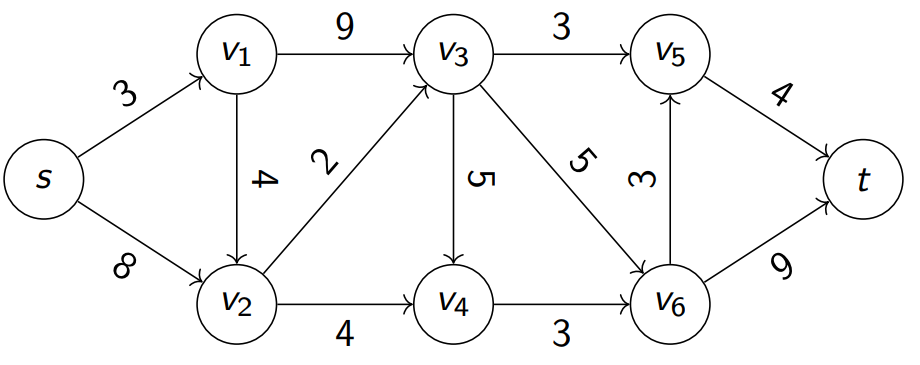
\includegraphics[width=0.5\linewidth]{flow}}
\caption{Example network flow graph.}
\label{flow}
\end{figure} 

\paragraph{Terminology}
\begin{itemize}
    \item \textbf{cut}: is a partition $(A, B)$ with $s \in A$ and $t \in B$
    \item \textbf{capacity} of a cut: $cap(A, B) = \sum_{e \, out \, from\, A} c(e)$
    \item \textbf{min-cut problem}: to find a cut of minimum capacity
    \item \textbf{flow} a function of how much of the capacity is used
    \item \textbf{capacity constraint} for each $e \in E, 0 \leq f(e) \leq c(e)$, an edge cannot have more flow than it's capacity
    \item \textbf{flow conservation constraint}: the flow coming in to a vertex $v$ must equal the flow going out from $v$, does not apply to source and sink.
    \item \textbf{maximum flow problem}: find a flow $f$ with maximum value
\end{itemize}

\par The \textbf{max-flow min-cut} theorem states that in the flow network you can calculate the maximum flow from $s$ to $t$ using the weight of the \textbf{minimum cuts}. That is, the weight of the edges that if removed would disconnect the source from the sink adds up to the maximum flow from $s$ to $t$.

\subsubsection{Ford-Fulkeson method}
The Ford-Fulkeson is a greedy algorithm that solves the \textbf{max-flow min-cut} problem. The main principle is to push as much flow up all edges until they are at their maximum. It terminates when no more flow can be pushed. If a BFS is used to search the graph it is called Edmonds-Karp's algorithm that has complexity $O(V^2 \cdot E)$

\par The running time of the Ford-Fulkeson algorithm is $O(E \cdot f)$ where $f$ is the maximum flow and $E$ is the number of edges because each augmenting path can be found in $O(E)$ time and increases the flow by an integer of at least 1, with the upper bound $f$. This can be improved upon with the fundamentally different \textbf{Preflow-Push} algorithm. This algorithm ignores the conservation constraint and instead creates a preflow which is modified until it becomes the maximum flow.

\begin{lstlisting}[language=Python, caption=Edmonds-Karp in Python]
# Returns the maximum flow from s to t in the given graph
    def EdmondsKarp(self, source, sink):
 
        # This array is filled by BFS and to store path
        parent = [-1] * (self.ROW)
 
        max_flow = 0 # There is no flow initially
 
        # Augment the flow while there is path from source to sink
        while self.BFS(source, sink, parent):
 
            # Find minimum residual capacity of the edges along the
            # path filled by BFS. Or we can say find the maximum flow
            # through the path found.
            path_flow = float("Inf")
            s = sink
            while s != source:
                path_flow = min(path_flow, self.graph[parent[s]][s])
                s = parent[s]
 
            # Add path flow to overall flow
            max_flow += path_flow
 
            # update residual capacities of the edges and reverse edges
            # along the path
            v = sink
            while v !=  source:
                u = parent[v]
                self.graph[u][v] -= path_flow
                self.graph[v][u] += path_flow
                v = parent[v]
 
        return max_flow
\end{lstlisting}

\begin{lstlisting}[language=Scala, caption=Preflow-Push in Scala]
def pushRelabel(graph: Graph, source: Int, sink: Int): Graph = {
        val n: Int = graph.length
        val resGraph: Graph = ArrayBuffer.fill(n, n)(0)
        val height: ArrayBuffer[Int] = ArrayBuffer.fill(n)(0) //height of node
        val excess: ArrayBuffer[Int] = ArrayBuffer.fill(n)(0) //flow into node minus flow from node
        val seen: ArrayBuffer[Int] = ArrayBuffer.fill(n)(0) //neighbours seen since last relabel
        //node "queue" n-2 because source and sink are not included
        val nodeList: ArrayBuffer[Int] = ArrayBuffer.fill(n)(0).zipWithIndex.map(t => t._2).filterNot(e => (e == source) || (e == sink))

        def push(u: Int, v: Int): Unit = {
            val send = scala.math.min(excess(u), graph(u)(v) - resGraph(u)(v))
            resGraph(u)(v) += send
            resGraph(v)(u) -= send
            excess(u) -= send
            excess(v) += send
        }

        def relabel(u: Int): Unit = {
            // find smallest new height making a push possible
            // if it exists at all
            var minHeight = Int.MaxValue / 3
            for (v <- 0 until n) {
                if ((graph(u)(v) - resGraph(u)(v)) > 0) {
                    minHeight = scala.math.min(minHeight, height(v))
                    height(u) = minHeight + 1
                }
            }
        }

        def discharge(u: Int): Unit = {
            while (excess(u) > 0) {
                if (seen(u) < n) { //check next neighbour
                    val v = seen(u)
                    if ((graph(u)(v) - resGraph(u)(v) > 0) && (height(u) > height(v))) {
                        push(u, v)
                    } else {
                        seen(u) += 1
                    }
                } else { //we have checked all neighbours. must relabel
                    relabel(u)
                    seen(u) = 0
                }
            }
        }

        height(source) = n
        excess(source) = Int.MaxValue / 3
        for (v <- 0 until n) {
            push(source, v)
        }

        var p = 0
        while (p < nodeList.length) {
            val u = nodeList(p)
            val oldHeight = height(u)
            discharge(u)
            if (height(u) > oldHeight) {
                nodeList.insert(0, nodeList.remove(p))
                p = 0
            } else {
                p += 1
            }
        }
        return resGraph
    }
\end{lstlisting}

\subsubsection{Special cases}

\paragraph{Maximum Edge-disjointed path}
Given a directed Graph $G(V, E)$ and two vertices $s$ and $t$ we want to find the maximum number of \textbf{edge-disjoint}, that is two paths that do not have two internal edges in common, paths from $s$ to $t$. This can be done by setting all capacities in the network except edges connected to either $s$ or $t$ to one.

\paragraph{Node independent path}
Given the directed graph $G(V, E)$ and two vertices $s$ and $t$ we want to find the maximum number of \textbf{vertex-independent} paths from $s$ to $t$. Again two paths are independent if they do not have two internal vertices in common, excluding $s$ and $t$. This is used to solve problems that require that each node is only able to be visited $x$ times. By splitting each node into two nodes and adding a capacity of one to the new edge we can guarantee that no node of the original graph is visited more than once as the ''internal'' capacity would be at it's maximum after the first pass.

\section{Complexity}
This section will cover notations and hardness of problems in this course.

\subsection{$O$, \Omega and \Theta}
We want to express hte growth rate of running times and other functions in a way that is insensitive ti constant factors and low-order terms. In ontehr words, we'd like to be able to take a running time like $1.62n^2 + 3.5n + 8$ and say that it grows like $n^2$ up to constant factors. 

\subsubsection{$O$}
Let $T(n)$ be a function, the worst-case runnig time of an algorithm for input $n$ for example. Given another function $f(n)$ we say that $T(n)$ is $O(f(n))$, read "$T(n)$ is order $f(n)$" if, for sufficently large $n$, the function $T(n)$ is bounded abouve by a constant multiple of $f(n)$. 
$O$ is a way to describe how algorithms grow as their input size grows, this can be applied to both running time and space requirement. When analysing algorithms you analyse how many times the different operations are run and find the dominating term. This way when the size of $n$ grows we can compare algorithms efficiency. If the algorithm is run in some complexity then all larger complexities is also applicable. Below is a table of the most common complexities in order.

\begin{table}[H]
\centering
\begin{tabular}{| c | c | c |}
    \hline
    Name & Complexity & Polyalgorithmic function \\
    \hline \hline
    Constant time & $O(1)$ & $-$ \\
    Log-logarithmic time & $O(log log n)$ & $T(n) = T(\sqrt{n})$\\
    Logarithmic time & $O(log(n))$ & $T(n) = T(\frac{n}{2})$ \\
    Linear time & $O(n)$ & $T(n) = T(n - 1) + T(n + 1)$ \\
    Quasilinear time & $O(n \cdot log(n))$ & $-$ \\
    Quadratic time & $O(n^2)$ & $T(n) = n + T(n -1)$ \\
    Exponential time & $O(2^n)$ & $-$ \\
    Factorial time & $O(n!)$ & $-$\\
    Example from lab & $O(2^{2^{n}})$ & $T(n) = (T(n-1))^2 \quad T(1) = 2$ \\
    \hline
\end{tabular}
\caption{Table of complexities and their corresponding polynomial description}
\label{table: 2}
\end{table}

\subsubsection{Memory complexity}
Big O notation in relation to memory denotes how memory allocation grows when the input $n$ grows. If for example we store a matrix of vertices and edges the complexity would be $O(n \cdot m)$. Commonly used in relation to dynamic programming.

\subsection{P, NP, NP-Complete \& NP-hard}

\paragraph{Decision and Optimization problems}
A decision problem is a problem that ask ''Does $X$ exist for $Y$?'' contrary to ''What is the $X$ of $Y$?''.

\paragraph{P}
$P$ is the complexity class that represent all problems that can be solved in \textbf{polynomial time}. All the algorithms in this class solves $P$ class problems.

\paragraph{NP}
$NP$, or non-deterministic polynomial, represents all the problems that can be checked but not necessarily solved in polynomial time. Note that $P \subseteq NP$.

\begin{figure}[H]
\center{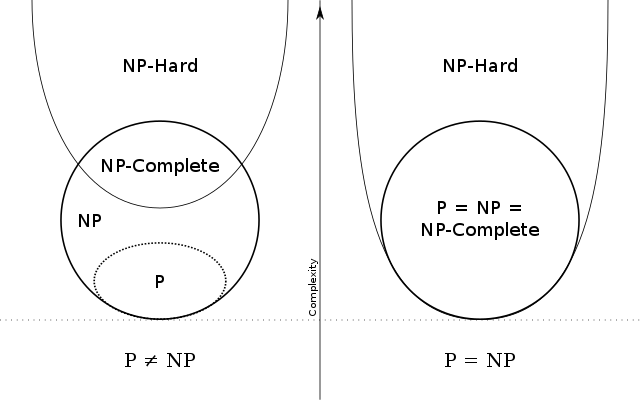
\includegraphics[width=0.5\linewidth]{np}}
\caption{Euler diagram for P, NP, NP-complete and NP-hard problems.}
\label{npProblems}
\end{figure} 

\paragraph{$P \neq NP$}
This is one of the millennium problems, The problem is to prove that some problems cannot be computed in polynomial time. This is \textbf{not} proven but many computer scientist think it is. To prove $P = NP$ would be ground breaking as many security algorithms rely on the fact that $P \neq NP$.

\subsubsection{NP-hard}
NP-hard problems really shouldn't be named as such, as there problems are not necessarily in $NP$ these problems are problems that are ''at least as hard as the hardest problems in $NP$''. More specifically a problem $X$ is considered NP-hard if each problem $Y \in NP$ can be reduced to $X$.

\subsubsection{NP-complete}
These problems exists in $NP$ which is described above. Consider a problem $X \in NP$, assume that each problem $Y \in NP$ can be reduced to $X$ then $X$ is NP-complete. Hence the two criteria for a problem to be NP-complete is.
\begin{itemize}
    \item $X \in NP$
    \item For all $Y \in NP$ we have $Y \leq_{p} X$
\end{itemize}
NP-complete problems are the hardest problems in $NP$, their class is $NPC$.

\subsubsection{Examples of NP-complete problems}

\paragraph{3-sat}
Is the problem of satisfying a given boolean formula, that is whether or not the variables of a given boolean formula can evaluate to TRUE. For example, the formula ''a AND NOT b'' is satisfiable because one can find the values a = TRUE and b = FALSE, which make (a AND NOT b) = TRUE. In contrast, ''a AND NOT a' is unsatisfiable.

\paragraph{Set cover}
Given a set of elements $S = {e_{1}, e_{2}, \dots, e_{n}}$ also called \textit{the universe} and a collection $M$ of sets $m$ whose union is equal to the universe. The problem is to find the smallest sub-collection of $M$ whose union equals the universe. Imagine boxes of LEGO with different pieces in them, $M$, how many boxes do i have to pick to build my desired LEGO ship?

\paragraph{Set Packing}
Given a finite set $S$ and a list of subsets of $S$. Then the set packing problem asks if some $k$ subsets in the list are \textbf{pairwise disjoint}. That is, no two of them share an element. 

\paragraph{3-dimentional matching}
This is a generalization of bipartite matching, 2-dimentional matching, to 3-dimentional hypergraphs.

\begin{figure}[H]
\center{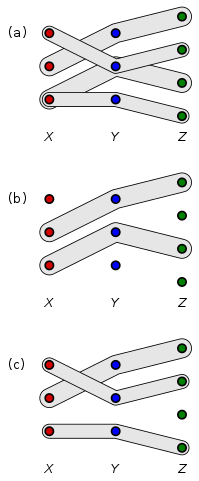
\includegraphics[width=0.5\textwidth,height=0.5\textheight,keepaspectratio]{3dim}}
\caption{Example 3-dim matching.}
\label{3dim}
\end{figure} 

\paragraph{Vertex cover}
Given a graph $G = (V, E)$ then set $S \subseteq V$ such that for every edge $(u, v) \in E$ we have ${u, v} \subseteq S$. That is, every edge $e \in E$ has at least one end in $S$. $S$ is called a \textbf{Vertex Cover}.

\par The NP-hard version of this problem, The minimum vertex cover, is the optimization and aims to find the smallest subset of vertices which reach all vertices in a graph 

\paragraph{Graph colouring}
This problem is in essence the labelling of elements in a graph with a certain constraint. In its simplest form we want to colour the vertices in a graph such that no two connected vertices share a colour. This problem is only NP-complete if the number of colours are larger than 3.

\par There is also the Graph Colouring Optimization problem, which is NP-hard. As even given a solution, you cannot say if is the minimum or not.

\paragraph{Hamiltonian Paths and Cycle}
Given a graph $G = (V, E)$ if you can traverse the graph and only visit any node one time then the graph contains a \textbf{Hamiltonian path}. A \textbf{Hamiltonian cycle} is a Hamiltonian path that terminates in the start node.

\par The NP-hard problem, Travelling salesman is the optimization of this problem.

\paragraph{Knapsack problem}
Given a set of items, each with a weight and value. Determine the number of items that maximizes the value with a weight $\leq$ a given limit.  

\par The optimization of this problem is, you guessed it, NP-hard. That is we want to find the optimal ration of value and weight.

\subsubsection{Examples of NP-hard problems}

\paragraph{Maximum independent set}
Given a graph $G = (V, E)$ and the nodes belong to a set $S$. The problem is to find the maximum set of nodes that are \textbf{independent}. Two nodes are independent if the nodes don't have an edge directly connecting them.

\paragraph{Travelling salesman problem}
Given a weighted graph, what is the shortest (minimum weight) path that visit each node and terminates in the start node.

\subsubsection{Identifying the degree of a problem}
Strategy for reduction:
\begin{itemize}
    \item Try to reduce to a known $P$ problem, otherwise step 2
    \item Try to reduce to a known NP-complete problem
    \item It's probably NP-hard
\end{itemize}

\paragraph{Reducing a problem}
If $Y \leq_{p} X$  then we can say that $Y$ is easy or that $X$ is hard. Hence to reduce a problem, if we can show that our problem is at least as hard as a known problem we can figure out how hard our problem is. So if you can reduce your problem to a NP-complete problem, you either have a NP-complete or NP-hard problem.

\par This is most commonly done by creating an instance of the NP-problem and with that instance create an instance of our problem. We can then conclude that if we have a solution to our problem that is also a solution to the NP-problem and hence our problem is equally as hard as the NP-problem.

\end{document}